

\setcounter{section}{2}
\section{System Components}
\bigskip

\subsection{MCU - ESP32}













\pagebreak
\subsection{Transceiver - DWM1000} 
\medskip
The Beacon and ID Tag communication will be done using ultra-wideband wireless communication. The most optimal transceiver available on the market that most fits the needs and scope of this project is the Decawave DWM1000 UWB module (Figure \ref{dwm1000}). The DWM1000 is an IEEE802.15.4-2011 UWB compliant and FCC/ETSI certified wireless transceiver module based on Decawave’s DW1000 IC \cite{R4-2-1}. This module is a combination of DW1000 IC, a built in antenna, power management system, and clock control for simple design integrations (Figure \ref{dwm1000_bd}). 

\medskip
\begin{figure}[H]
\centering
    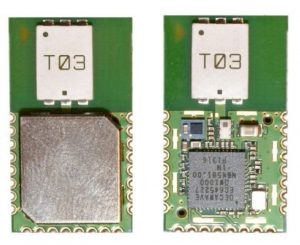
\includegraphics[scale=0.75]{./images/dwm1000.jpg}
    \caption{Decawave DWM1000 Modules}
    \label{dwm1000}
\end{figure}

The module enables the location tracking of objects in real time location systems (RTLS) to a precision of 10 cm indoors. It supports high range of communications data rates from 110 Kbps up to 6.8 Mbps, with excellent communication ranges of up to 300m. The frequencies of operation in the range of 3.5 GHz to 6.5 GHz with seven distinct channels which would significantly reduce issues of signal interference or multipath propagation. Its small physical size allows the module to be implemented in highly cost-effective solutions. By using this modul,e integration with the Akriveia Beacon system is intuitive and simple; since the DWM1000 also offers a wide range of MCU support such as Arduino MCUs or the ESP32 MCUs. 

\medskip
\begin{figure}[H]
\centering
    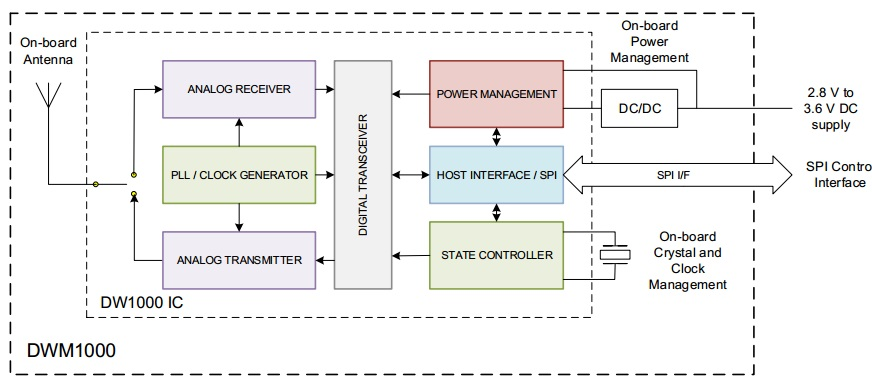
\includegraphics[scale=0.7]{./images/dwm1000_bd.jpg}
    \caption{DWM1000 Internal Block Diagram}
    \label{dwm1000_bd}
\end{figure}






\pagebreak
\subsection{DPU - Raspberry Pi}







